% Syslab Research Journal Template
% By Patrick White
% September 2019

% Do not edit this header
\documentclass[letterpaper,11pt]{article}
\usepackage{fullpage}
\usepackage{palatino}
\usepackage{courier}
\usepackage{graphicx}
\def\hrulefill{\leavevmode\leaders\hrule height 20pt\hfill\kern\z@}

% ------------- Edit these definitions ---------------------
\def\name{Bryan Lu}
\def\journalnum{6}
\def\daterange{10/7/19-10/14/19} % starts on Monday
\def\period{2}
% ------------------ END ---------------------------------
% Do not edit this
\begin{document}
	\thispagestyle{empty}
	\begin{flushright}
		{\Large Journal Report \journalnum} \\
		\daterange\\
		\name \\
		Computer Systems Research Lab \\
		Period \period, White
		\end{flushright}
	\hrule height 1pt

% ------ SECTION DAILY LOG -------------------------------------
\section*{Daily Log}
%Detail for each day about what you research, coded, debug, designed, created, etc. Informal style is OK.
\vspace{-0.7em}

\subsection*{Monday, October 7}
\vspace{-0.5em}
I quickly added Greek-letter functionality to the part of my code that can identify explicit variables, and reread the original paper to discern what kinds of properties the language needed. 
\vspace{-1.0em}
\subsection*{Tuesday, October 8}
\vspace{-0.5em}
I figured out what the relations actually were in my problem, and what properties they needed to have, and I started to create a dictionary with detected words mapping to objects and relations. 
%% relations -> turn them into names of actual functions, determine return type for them, whether they are unary/binary, explicit/implicit variable, word distance of objects, 
\vspace{-1.0em}
\subsection*{Thursday, October 10}
\vspace{-0.5em}
I created \texttt{lexicon.txt}, a file with words to detect for and corresponding objects and relations, and continued to fill in the corresponding relations and objects for various words. 
% ------ SECTION TIMELINE -------------------------------------
%\newpage
\vspace{-1.7em}
\section*{Timeline}
\begin{tabular}{|p{1in}|p{2.5in}|p{2.5in}|}
	\hline 
9/23 & Filter posts that are not standard olympiad geometry problems, and construct a standard lexicon of keywords to look for in a problem both as objects and as relations. & Yes, I created two separate files for various geometrical objects and relations that I found that appeared in my data set. \\
	\hline
9/30 & Write code that creates a graph structure corresponding to the problem statement, with objects as nodes and relations as edges. & My code definitely is able to identify all the nodes/concepts and what kinds of relations are present in the problem, but not much more.  \\
	\hline
10/7 & Create a logical language to give more structure and properties to the objects and relations detected in the problem.  & Not quite the goal I needed to meet, but I figured out the path I need to take going forward and started creating the dictionary I needed to have for my problem. \\
	\hline 
10/14 & Finalize the object identification associated with \texttt{lexicon.txt}, and figure out how to extract the necessary data to pass to the log-linear classifier later. & N/A \\
	\hline 
10/21 & Research how to write code to create a log-linear classifier using \texttt{scikit}, and create some sort of working learning algorithm. & N/A \\
	\hline 
\end{tabular}


% ------ SECTION REFLECTION  ---------------------------------
\section*{Reflection}
%In narrative style, talk about your work this week. Successes, failures, changes to timeline, goals. This should also include concrete data, e.g. snippets of code, screenshots, output, analysis, graphs, etc.

I finally figured out the approach I needed to take to making progress in my project this week. I've begun creating a system for myself -- for every word that appears in the text that is geometrically relevant, I'm going to associate with it all the possible objects and relations that can go with it. The objects are the strings that start with a lowercase letter, and the relations look like Java methods and start with an uppercase letter: 
\begin{center}
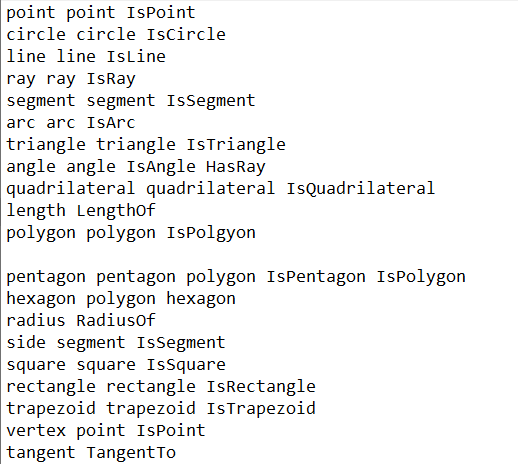
\includegraphics[scale=0.5]{lexicon.png}
\end{center}
This is admittedly incomplete, but this is what I'm looking for, but for all geometrically-associated words.

I also began to think about creating training data for my machine learning model, which would require me to list what explicit relations are valid for each problem. Looking over my problems/data set once more this week, I found that a lot of them are fairly arbitrary in their configurations, which would make my job to confidently determine which relations are correct for each problem much harder. I'll need to keep this in mind as the end goal for this stage of the process. 



\end{document}

